\begin{example}[Advection-diffusion 2D]
\label{ex:quart3}
Based on Example 3 in \cite{Antonietti2013},
in $\Omega = \langle 0, 1 \rangle^2$ we will once again solve equation
%\begin{equation}
%	\pdiff{u}{x} + \pdiff{u}{y} - D \cdot \left( \pdiff{^2 u}{x^2} + \pdiff{^2 
%	u}{y^2} \right) = g
%\end{equation}
%i.e
%\begin{equation}
%	\vec{a} \cdot \nabla u - D \Delta u = g
%\end{equation}
%where $\vec{a} = [1, 1]^T$ is advection velocity and $D$ is diffusion 
%coefficient and $g$ is a source function.
We set up boundary condition and source function in such a way that the exact 
solution $u_{exact}$ is
\begin{equation}
	u_{exact} = -xy + x +y + \frac{\exp{\left(-\frac{{\left(x - 1\right)} {\left(y - 
	1\right)}}{D}\right)} - 
	\exp{\left(-\frac{1}{D}\right)}}{\exp{\left(-\frac{1}{D}\right)} 
	- 1}.
\end{equation}
We omit analytical forms of $g$ and boundary conditions for brevity, they can found in 
the code. Different values of 
coefficient $C_w$ in penalty term yield different convergence behavior as 
demonstrated in Figure 
\ref{fig:conv_qart3} and \Cref{fig:orders_quarteroni3}
\end{example}

\begin{figure}[h!]
	\centering
	\begin{tabular}{p{0.5\textwidth} p{0.5\textwidth}}
	\vspace{0pt} 
	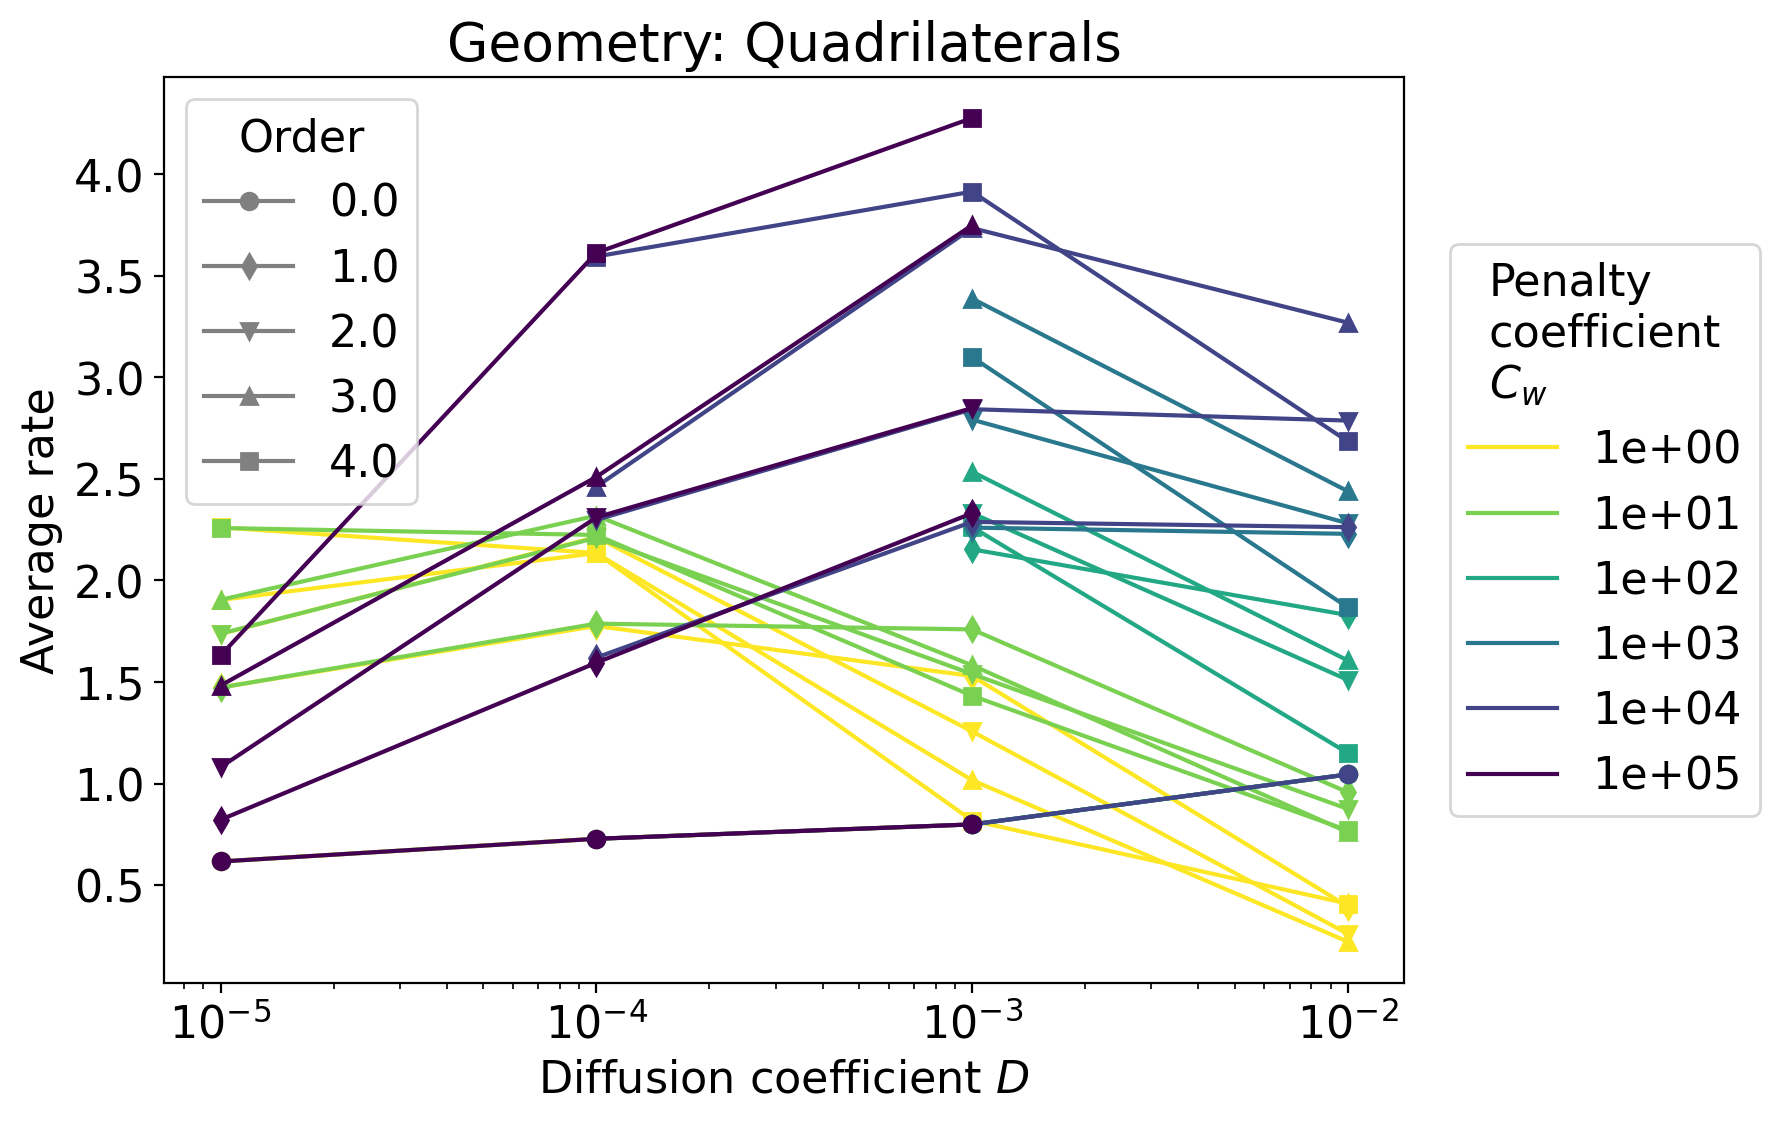
\includegraphics[width=0.49\textwidth]{../figs/parametric/advdiff_2D/ord_quarteroni2_2_4}
	&
	\vspace{0pt} 
	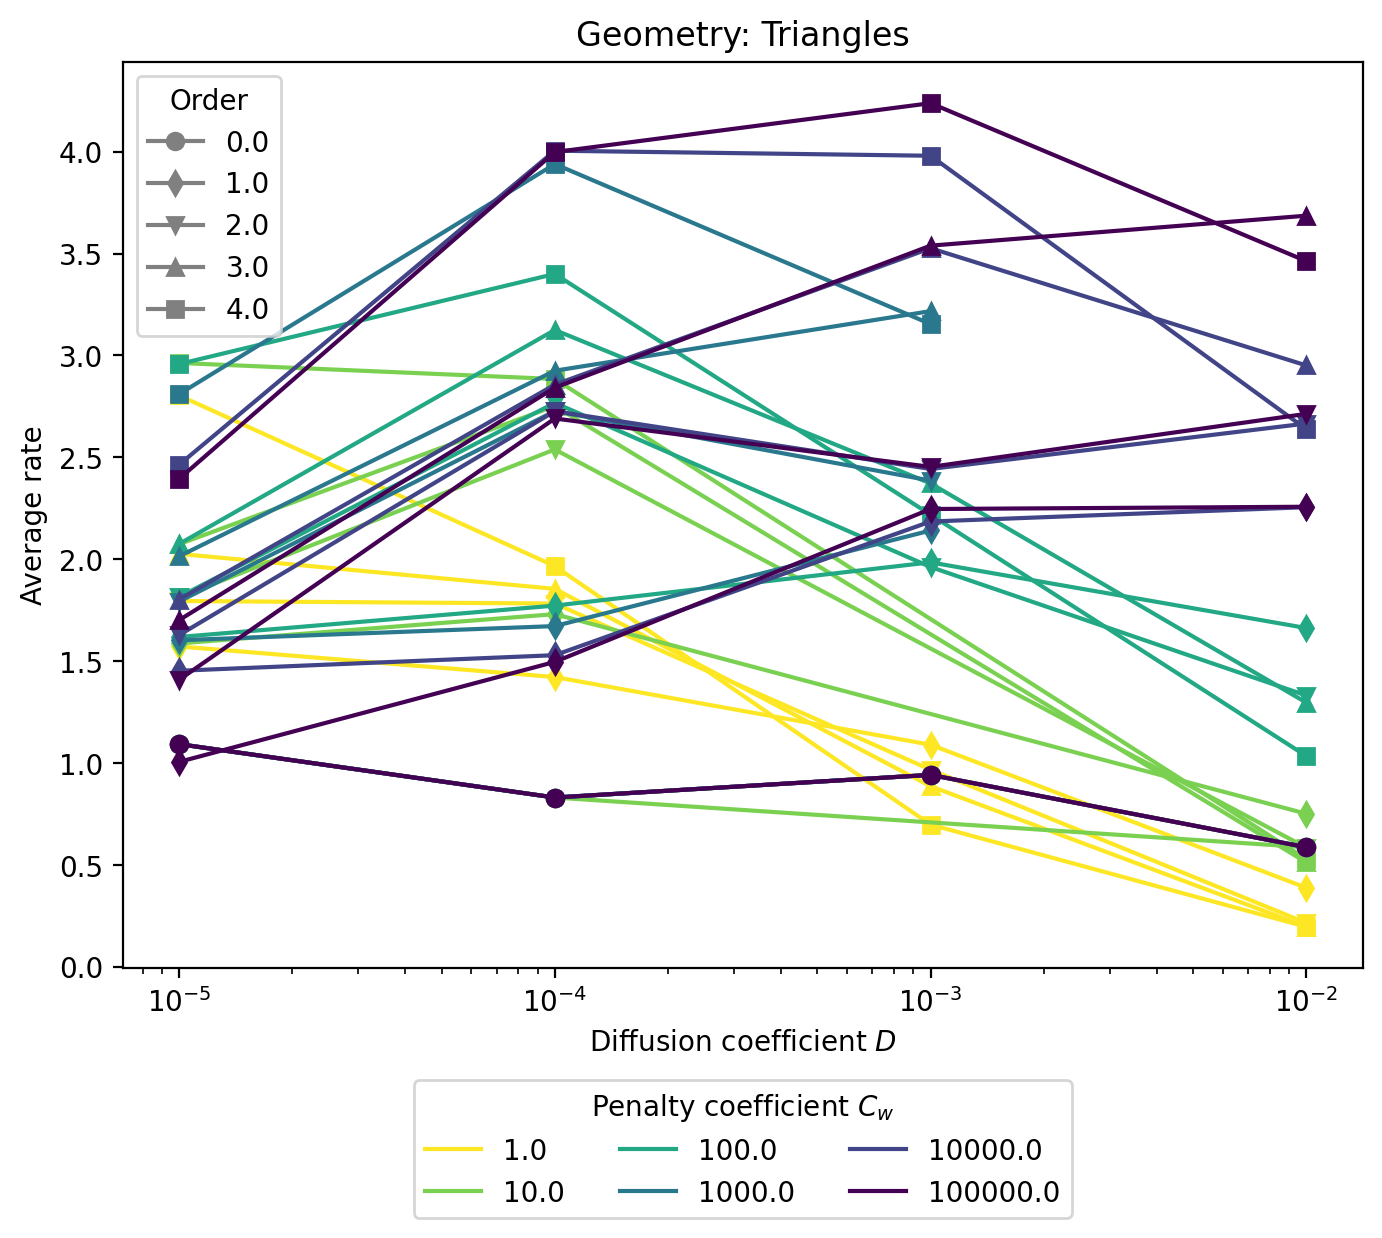
\includegraphics[width=0.49\textwidth]{../figs/parametric/advdiff_2D/ord_quarteroni2_2_3}
	\end{tabular}
	\caption{\Cref{ex:quart3} average order for different choice of $C_w$}
	\label{fig:orders_quarteroni3}
\end{figure}


\begin{figure}[p!]
	\centering
	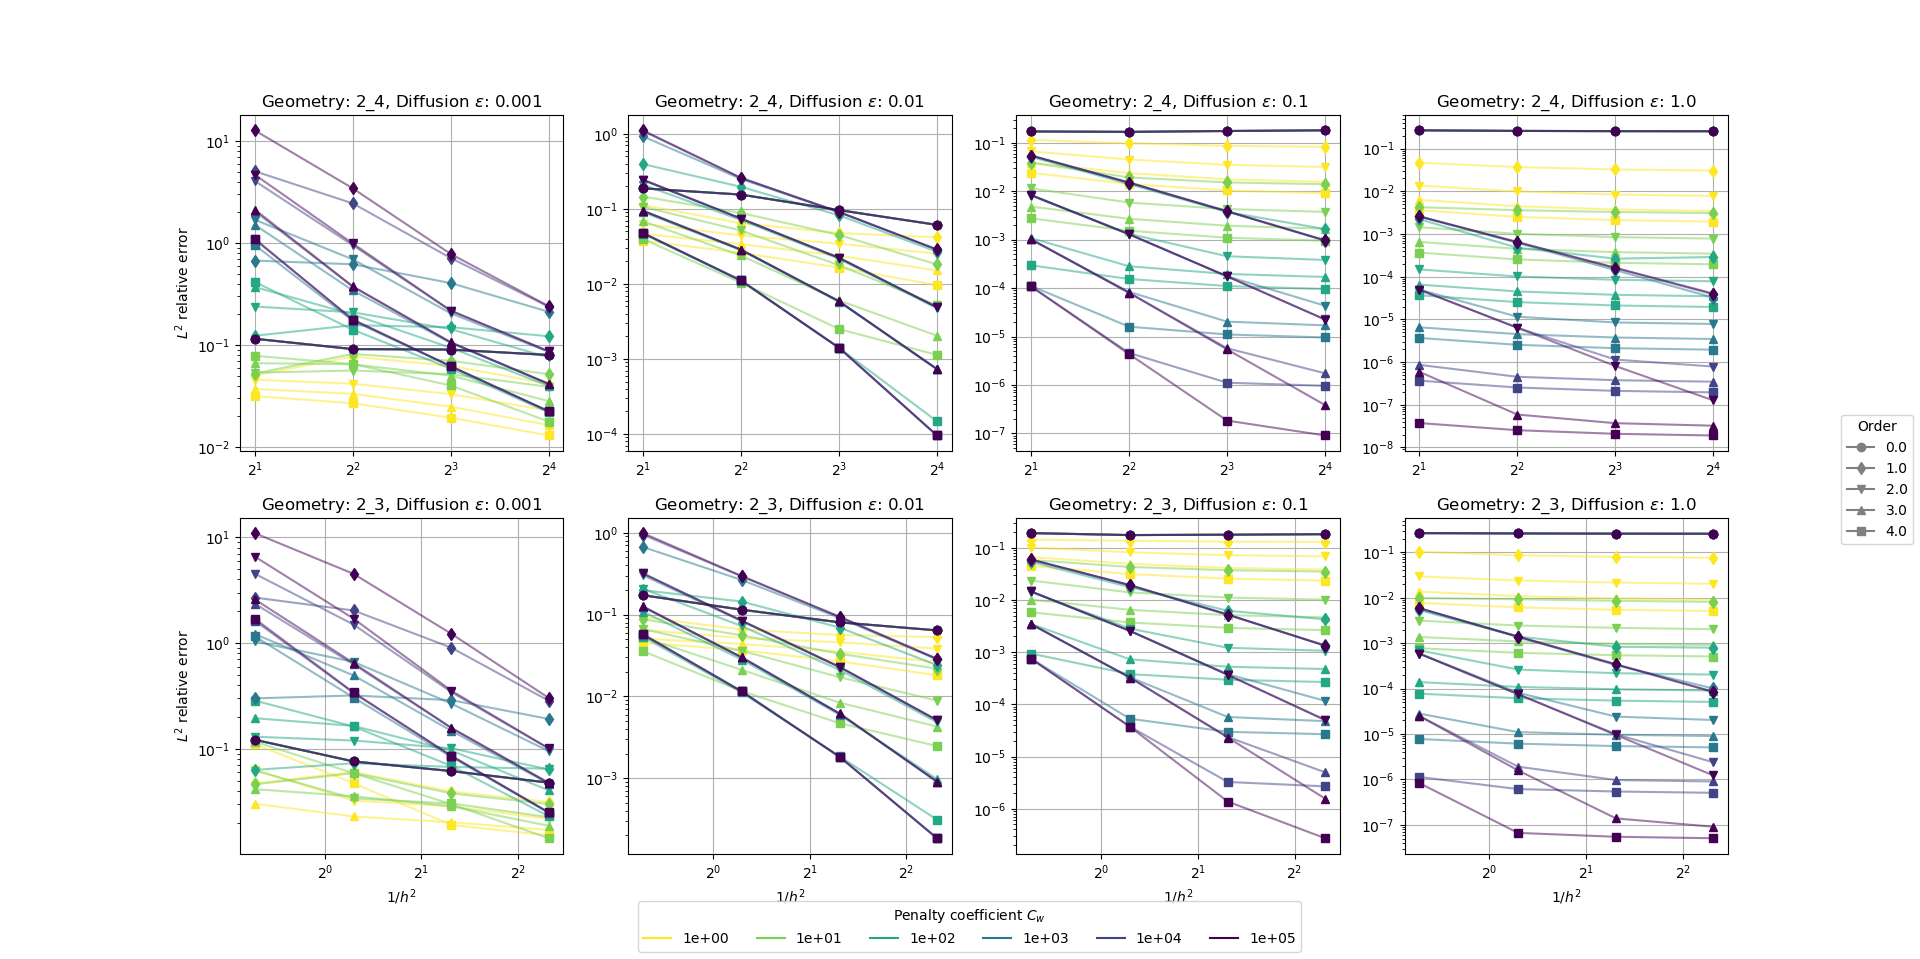
\includegraphics[height=\textheight]{../figs/parametric/advdiff_2D/quarteroni3.png}
	
	\caption{\Cref{ex:quart3} convergence graphs for different choice of $C_w$}
	\label{fig:conv_qart3}
\end{figure}